% !TEX program = xelatex
\documentclass[10pt,letterpaper,twocolumn]{article}

% === GEOMETRY ===
\usepackage[top=0.75in, bottom=0.75in, left=0.75in, right=0.75in]{geometry}

% === FONTS ===
\usepackage{fontspec}
\setmainfont{Latin Modern Roman}[
  Extension=.otf,
  UprightFont=lmroman10-regular,
  BoldFont=lmroman10-bold,
  ItalicFont=lmroman10-italic,
  BoldItalicFont=lmroman10-bolditalic,
]
\setsansfont{Latin Modern Sans}[
  Extension=.otf,
  UprightFont=lmsans10-regular,
  BoldFont=lmsans10-bold,
  ItalicFont=lmsans10-oblique,
  BoldItalicFont=lmsans10-boldoblique,
]
\setmonofont{Latin Modern Mono}[
  Extension=.otf,
  UprightFont=lmmono10-regular,
  ItalicFont=lmmono10-italic,
  Scale=0.85,
]
% YWFT Processing carries the display title only. Its punctuation glyphs
% are unreliable and its charset omits dashes, so nothing with a mark in
% it is ever set in this face.
\newfontfamily\acbold{ywft-processing-bold}[
  Path=../../system/public/type/webfonts/,
  Extension=.ttf
]

% === PACKAGES ===
\usepackage{xcolor}
\usepackage{titlesec}
\usepackage{enumitem}
\usepackage{booktabs}
\usepackage{tabularx}
\usepackage{fancyhdr}
\usepackage{hyperref}
\usepackage{xurl}
\usepackage{graphicx}
\usepackage{ragged2e}
\usepackage{microtype}
\usepackage{natbib}
\usepackage{tikz}
\usetikzlibrary{positioning,arrows.meta,calc,shapes.geometric}
\usepackage{../ac-source-bundle}

% === COLORS ===
\definecolor{acpink}{RGB}{180,72,135}
\definecolor{acpurple}{RGB}{120,80,180}
\definecolor{acdark}{RGB}{64,56,74}
\definecolor{acgray}{RGB}{119,119,119}
\definecolor{acgreen}{RGB}{46,150,72}
\definecolor{acblue}{RGB}{54,110,190}
\definecolor{acamber}{RGB}{201,138,20}

% === HYPERREF ===
\hypersetup{
  colorlinks=true,
  linkcolor=acpurple,
  urlcolor=acpurple,
  citecolor=acpurple,
  pdfauthor={@jeffrey},
  pdftitle={Who Is Painting},
}

% === SECTION FORMATTING ===
\titleformat{\section}
  {\normalfont\bfseries\normalsize\uppercase}
  {\thesection.}
  {0.5em}
  {}
\titlespacing{\section}{0pt}{1.2em}{0.3em}
\titleformat{\subsection}
  {\normalfont\bfseries\small}
  {\thesubsection}
  {0.5em}
  {}
\titlespacing{\subsection}{0pt}{0.8em}{0.2em}

% === HEADER/FOOTER ===
\pagestyle{fancy}
\fancyhf{}
\renewcommand{\headrulewidth}{0pt}
\fancyhead[C]{\footnotesize\color{acgray}\textit{Who Is Painting}}
\fancyfoot[C]{\footnotesize\thepage}

% === LISTS, COLUMNS, PARAGRAPHS ===
\setlist[itemize]{nosep, leftmargin=1.2em, itemsep=0.15em}
\setlist[enumerate]{nosep, leftmargin=1.4em, itemsep=0.15em}
\setlength{\columnsep}{1.8em}
\setlength{\parindent}{1em}
\setlength{\parskip}{0.3em}
\tolerance=800
\emergencystretch=1em
\hyphenpenalty=50

% === BRAND ===
\newcommand{\acdot}{{\color{acpink}.}}
\newcommand{\ac}{Aesthetic{\acdot}Computer}

% === TIKZ STYLES ===
\tikzset{
  band/.style={draw=acgray!60, line width=0.5pt, fill=white,
               inner sep=0pt, font=\scriptsize\sffamily, text=acdark, align=center},
  tag/.style={font=\scriptsize\sffamily, text=acgray, align=left},
  tagr/.style={font=\scriptsize\sffamily, text=acgray, align=right},
}

\begin{document}

\twocolumn[{%
\begin{center}
{\acbold\fontsize{27pt}{31pt}\selectfont\color{acdark} Who Is Painting}\par
\vspace{0.55em}
{\itshape\fontsize{13pt}{16pt}\selectfont\color{acpink}
An investigation of 331 No Paint paintings that arrived in two school mornings}\par
\vspace{0.6em}
{\small\color{acgray} \href{https://prompt.ac/@jeffrey}{@jeffrey} \,$\cdot$\, \ac{} \,$\cdot$\, ORCID \href{https://orcid.org/0009-0007-4460-4913}{0009-0007-4460-4913}}\par
\vspace{0.25em}
{\small\color{acgray} 4 November 2026}\par
\vspace{0.55em}
{\color{acpink}\rule{\textwidth}{1.2pt}}
\vspace{0.5em}
\end{center}

\begin{quote}
\small\noindent\textbf{Abstract.}
On Monday 2~November 2026, visits to \texttt{nopaint.art}, the home of
the 2016 painting game No Paint, rose from about 18 a day to more than
400. The first explanation was search traffic, and the first measure of
it was wrong: the first-party visit collector showed no paintings being
saved, because the 2021 build saves through its own endpoint, which that
collector never sees. Reading the endpoint's database directly showed
\textbf{331} paintings saved with \emph{Done} in 48 hours, against a
prior rate of about three a day. They arrived in four blocks of 80 to
100 minutes starting at 8:15 and 11:30 on Tuesday and Wednesday,
Lima time. The access log still held 146 of Wednesday's uploads; all
came from Peruvian networks, and eight came from an address whose
reverse DNS names a school's \texttt{.edu.pe} domain. This paper records
the investigation as it happened, including its two wrong turns, tests
one competing explanation (judging for the .ART Award) and rejects it,
and describes the instruments built the same day to answer the next
questions: a 50/50 sticker test, a funnel for the AI studio
\texttt{notepaint.art}, and a bilingual note form for teachers.
\end{quote}
\vspace{0.5em}
}]

\section{Introduction}

The question that started this was casual: what did the network do
overnight? The answer was a single outlier. Of 625 page visits across
the \ac{} network in the twelve hours to 9:50am Pacific on
4~November, 405 were to \texttt{nopaint.art}, and 86\% of those
visitors touched the canvas. The site had averaged fewer than
twenty visits a day the week before.

No Paint is a painting game from 2016, made with Alex Freundlich, Ella
Fleck, Camille Klein and friends~\citep{scudder2016nopaint}. A painting
grows one proposed mark at a time and the player answers \emph{Paint} or
\emph{No}. The 2021 build, made in Construct, still runs at
\texttt{nopaint.art}; it was refreshed in 2026 as the entry for the
.ART Award~\citep{dotart2026award}. Its AI successor,
\texttt{notepaint.art}, lives beside it, and since 2~November a
sticker on No Paint's title screen has pointed at it.

The investigation asked four questions in turn. Who were the visitors?
Were they making anything? Where were they? What would we need in place
to learn more without guessing? Each section below answers one, in the
order the answers came. It follows the network traffic report~\citep{scudder2026traffic} and
the earlier network audit~\citep{scudder2026audit} in posture: every
number comes from a primary pull. Two early answers were wrong, and both are kept,
because how they went wrong describes the instruments better than a
clean account would.

\section{Instruments}
\label{sec:instruments}

Six sources were read. They differ in what they can see, and most of
this paper turns on those differences.

\begin{itemize}
\item \textbf{Visit collector.} A first-party script on every studio
domain posts one cumulative record per page visit: surface, dwell
bucket, whether the visitor interacted, a referrer \emph{host}, and a
fixed allowlist of milestone actions. It keeps no identifiers and
expires rows after 35 days. It counts AC's own media saves but not the
2021 game's.
\item \textbf{Search Console.} Google's clicks and impressions for
\texttt{nopaint.art}, lagging two days~\citep{google2026performance}.
\item \textbf{The classic save endpoint.} \emph{Done} in the 2021 build
reserves an eight-character code from \texttt{server.nopaint.art}, then
posts the PNG. On lith, the server behind the network, the host is
rewritten to a function that stores each painting in the Mongo
collection \texttt{nopaint-classic-paintings} with a \texttt{savedAt}
time. Each saved painting is public at
\texttt{server.nopaint.art/painting/<code>.png}.
\item \textbf{The access log.} Caddy writes JSON lines for every request
to lith~\citep{caddy2026log}. It rolls at 50\,MiB and keeps three files
for at most 72~hours, so on a busy server its memory is shorter than
three days.
\item \textbf{notepaint's public sitemap.} Every saved notepaint
painting is public by design, with its note in the page title.
\item \textbf{AC's recent-paintings feed.} The public list behind
\texttt{aesthetic.computer}'s \texttt{done} command.
\end{itemize}

\section{The spike}
\label{sec:spike}

Table~\ref{tab:visits} gives \texttt{nopaint.art}'s visits in 24-hour
windows ending at 18:38\,UTC. The jump falls inside the window that
opens Monday morning in the Americas, and it is not a bot artifact:
the collector marked one automated visit in the last 24~hours, and 85\%
of human visits were engaged, meaning they interacted and stayed
visible for at least ten seconds.

\begin{table}[t]
\centering\small
\caption{Page visits to \texttt{nopaint.art} from the first-party
collector. Engaged means interacted and visible for 10\,s or more.}
\label{tab:visits}
\begin{tabular}{@{}lrr@{}}
\toprule
24-hour window ending 18:38 UTC & Visits & Engaged \\
\midrule
29 Oct--1 Nov (per day, mean of 3) & 18 & 7 \\
2 Nov & 36 & 19 \\
3 Nov & 337 & 292 \\
4 Nov & 440 & 372 \\
\bottomrule
\end{tabular}
\end{table}

In the twelve-hour window, 154 visits arrived with \texttt{google.com}
as referrer and 195 with \texttt{nopaint.art} itself, which is what a
reload or a return to the page produces. Search Console showed about two
clicks a day for the site through 2~November, the last day it had. That
gap was the first open question: either Search Console had not caught
up, or the visits were coming from a Google surface that does not count
as a search click, such as Discover~\citep{google2026discover}. It is
still open; Search Console's data for the spike days had not arrived
when this was written.

\subsection{First wrong turn: nobody is making anything}

The collector's milestone counts showed no saved-painting
action on \texttt{nopaint.art} or \texttt{aesthetic.computer} during
the spike, and AC's public paintings feed showed one upload, from a
regular. The first report concluded that the visitors were not making
paintings, and supported it by searching the 2021 build's project file
for an upload URL and finding none.

Both supports were wrong. The project file stores event logic as
numeric references into a compiled expression table, so the URLs are
not in it as plain strings; they live in the runtime script, where
\texttt{server.nopaint.art/upload-painting} appears in the clear. And
the collector counts AC's own media saves, which the 2021 game does not
use. The correction came from the person who wrote the save path. The
lesson is narrower than ``check your work'': an absence in an instrument
is only evidence if the instrument could have seen the thing.

\section{What was made}
\label{sec:made}

Read directly, the classic endpoint's collection held 331 paintings
saved between 10:21am Pacific on 2~November and 10:15am Pacific on
4~November (Figure~\ref{fig:perday}). The thirteen days from
20~October to 1~November had averaged 4.3 a day. Only one code was reserved by \emph{Done} and not completed
in the last 24 hours, so almost every attempt to save succeeded.

\begin{figure}[t]
\centering
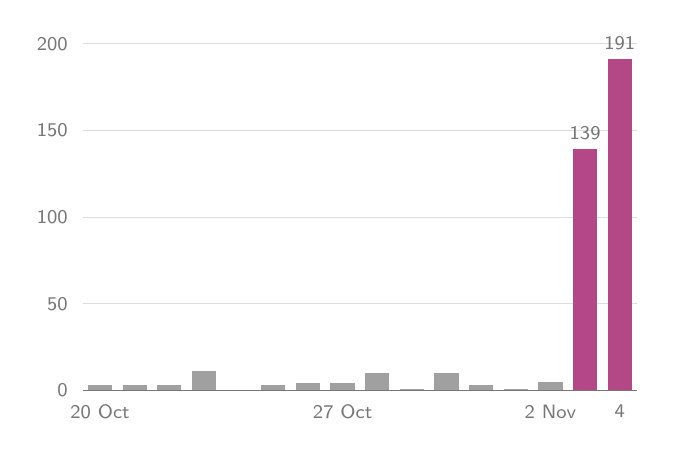
\begin{tikzpicture}[x=0.44cm,y=0.022cm]
  \foreach \y in {0,50,100,150,200} {
    \draw[acgray!25, line width=0.3pt] (0,\y) -- (16,\y);
    \node[tagr, anchor=east] at (-0.15,\y) {\y};
  }
  \foreach \i/\n in {0/3,1/3,2/3,3/11,4/0,5/3,6/4,7/4,8/10,9/1,10/10,11/3,12/1,13/5} {
    \fill[acgray!70] (\i+0.15,0) rectangle (\i+0.85,\n);
  }
  \fill[acpink] (14.15,0) rectangle (14.85,139);
  \fill[acpink] (15.15,0) rectangle (15.85,191);
  \node[tag, anchor=south] at (14.5,139) {139};
  \node[tag, anchor=south] at (15.5,191) {191};
  \draw[acgray, line width=0.4pt] (0,0) -- (16,0);
  \node[tag, anchor=north] at (0.5,-3) {20 Oct};
  \node[tag, anchor=north] at (7.5,-3) {27 Oct};
  \node[tag, anchor=north] at (13.5,-3) {2 Nov};
  \node[tag, anchor=north] at (15.5,-3) {4};
\end{tikzpicture}
\caption{Paintings saved with \emph{Done} in the 2021 No Paint, per UTC
day. The 4~November bar covers the day to 18:15\,UTC.}
\label{fig:perday}
\end{figure}

Figure~\ref{fig:sheet} shows all 331 in save order. They are not test
images or repeated blanks. They look like No Paint paintings always
have: noisy grounds, stamped shapes, filters, the occasional face or
word, each one the result of dozens of accepted and rejected proposals.
A handful are near-duplicates saved seconds apart, which is what two
students at one screen produce.

\begin{figure*}[t]
\centering
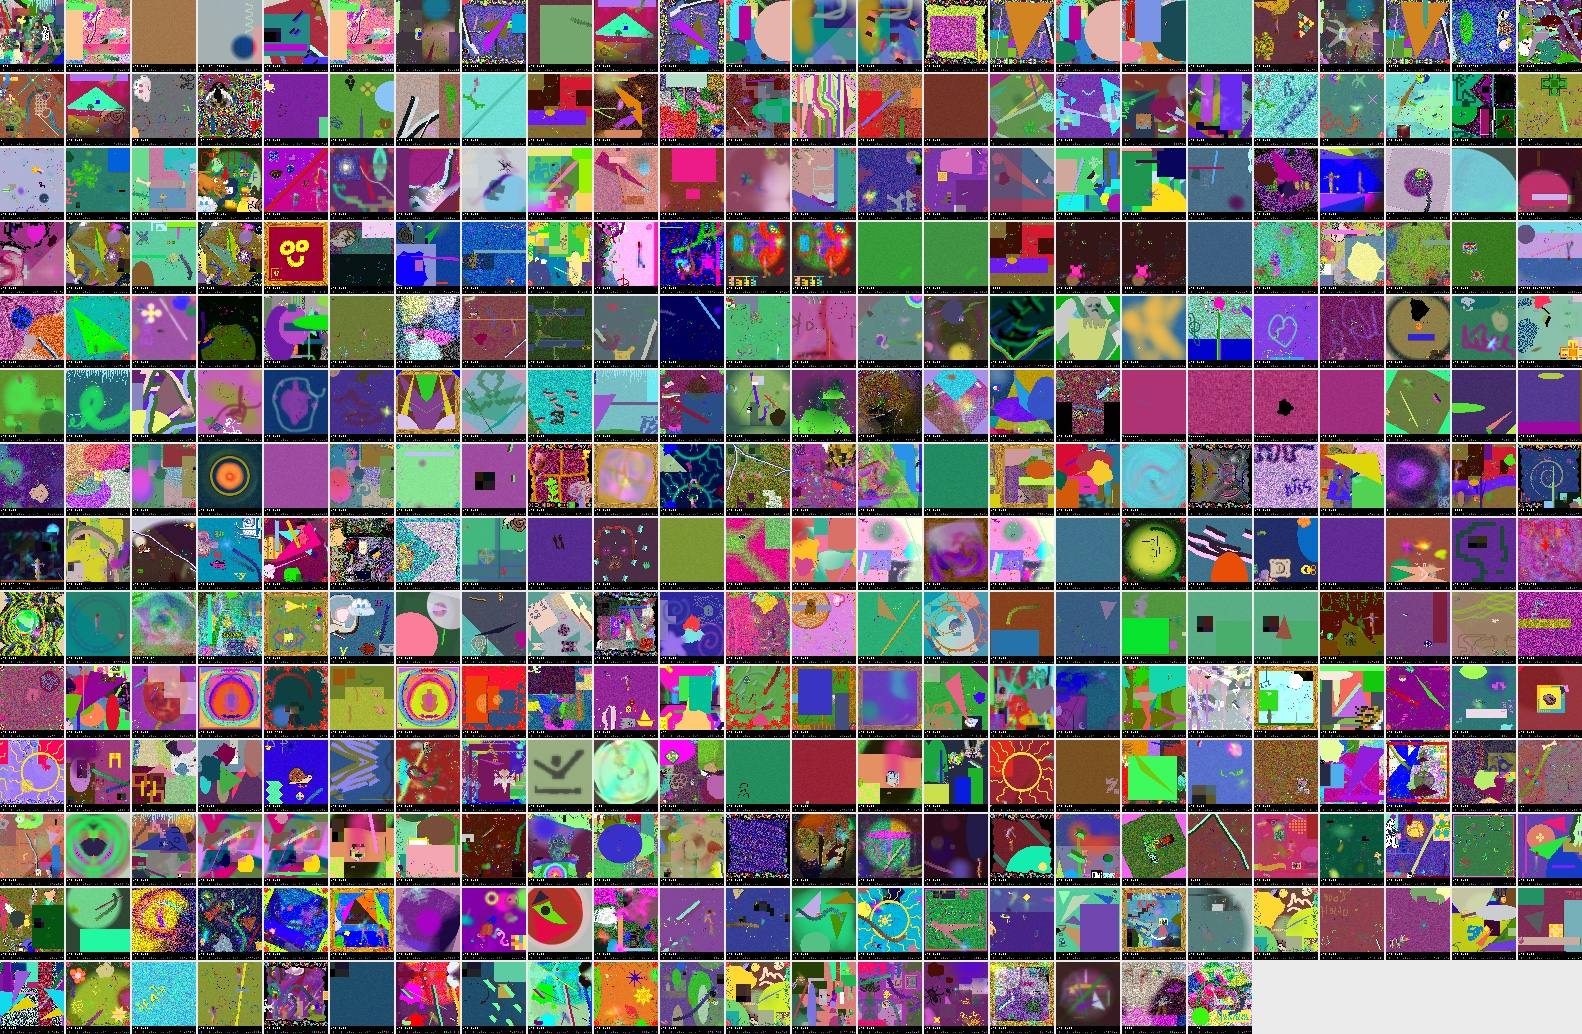
\includegraphics[width=\textwidth]{figures/paintings-sheet.jpg}
\caption{The 331 paintings saved with \emph{Done} from 2~November 18:21\,UTC
to 4~November 18:15\,UTC, in save order, left to right and top to bottom.
Each tile is the saved PNG scaled to 64\,$\times$\,72 pixels. Every image
is public at \texttt{server.nopaint.art}; none carries a name.}
\label{fig:sheet}
\end{figure*}

\subsection{The shape of the arrivals}

The saves are not spread across the day. Grouped by gaps of more than
25 minutes, 322 of the 331 fall into four blocks (Figure~\ref{fig:hours}):
79 saves from 8:17 to 9:49 and 52 from 11:32 to 12:54 on Tuesday, then
111 from 8:15 to 9:00 and 80 from 11:36 to 13:15 on Wednesday, all in
Lima time (UTC$-$5). The busiest ten minutes held 38 saves. Nothing
arrived on either evening.

\begin{figure}[t]
\centering
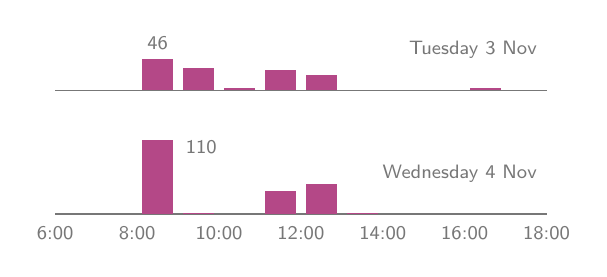
\begin{tikzpicture}[x=0.52cm,y=0.0085cm]
  % Tuesday row at y=0, Wednesday row offset by 150 units
  \foreach \row/\off/\lab in {Tue/185/Tuesday 3 Nov, Wed/0/Wednesday 4 Nov} {
    \draw[acgray, line width=0.4pt] (0,\off) -- (12,\off);
    \node[tag, anchor=east] at (12,\off+60) {\lab};
  }
  \foreach \h/\n in {2/46,3/33,4/3,5/30,6/22,10/3} {
    \fill[acpink] (\h+0.12,185) rectangle (\h+0.88,185+\n);
  }
  \foreach \h/\n in {2/110,3/1,5/34,6/45,7/1} {
    \fill[acpink] (\h+0.12,0) rectangle (\h+0.88,\n);
  }
  \node[tag, anchor=south] at (2.5,185+46) {46};
  \node[tag, anchor=west] at (2.95,100) {110};
  \foreach \h/\t in {0/6,2/8,4/10,6/12,8/14,10/16,12/18} {
    \node[tag, anchor=north] at (\h,-4) {\t:00};
  }
\end{tikzpicture}
\caption{Saves per hour on the two school days, Lima time. Each bar is
one clock hour. The four class blocks start at about 8:15 and 11:30.}
\label{fig:hours}
\end{figure}

Lima time is not a guess fitted to the bars. It came from the next
measurement, and the clock fit afterwards: two blocks a day, starting at
8:15 and 11:30, of about one class period each, on consecutive weekdays.

\section{Where they were}
\label{sec:where}

The access log no longer reached Tuesday, but it still held 146 of
Wednesday's 191 saves. Each request's address was mapped to the owner
of its network through Team Cymru's public DNS service~\citep{cymru2026asn}
and to a reverse-DNS domain. The script printed only network names,
domains and counts; no address was printed or kept. Table~\ref{tab:nets}
is the whole result.

\begin{table}[t]
\centering\small
\caption{Networks behind the \texttt{POST /upload-painting} requests
still in the access log on 4~November (oldest line 13:36\,UTC). Addresses
is the number of distinct source addresses.}
\label{tab:nets}
\begin{tabular}{@{}lrr@{}}
\toprule
Network & Uploads & Addresses \\
\midrule
Integratel Per\'u (AS6147) & 72 & 11 \\
Am\'erica M\'ovil Per\'u, Claro (AS12252) & 43 & 7 \\
Entel Per\'u (AS21575) & 23 & 6 \\
A school's network (\texttt{.edu.pe}) & 8 & 1 \\
\midrule
Total & 146 & 25 \\
\bottomrule
\end{tabular}
\end{table}

Every upload came from Peru. Three of the four networks are national
mobile and home carriers, which do not identify who is behind them. The
fourth is a business line whose address resolves to a school's own
\texttt{.edu.pe} domain: a Catholic school in metropolitan Lima. That
is the only institution the data names, and it accounts for eight
uploads from a single address. Twenty-five addresses for 146 paintings
is about six paintings per address, which fits shared classroom
connections or phones on a school's carrier better than one student per
device.

What the data supports is narrow. Students in Lima, in at least one
school and possibly several, used No Paint in morning class periods on
Tuesday and Wednesday. One school is identified. Whether its class made
most of the 331 paintings or only eight of them, the log cannot say.

\begin{table*}[t]
\centering\small
\caption{Instruments added on 4~November 2026, and the question each one answers.}
\label{tab:features}
\begin{tabularx}{\textwidth}{@{}>{\raggedright\arraybackslash}p{0.25\textwidth}>{\raggedright\arraybackslash}X>{\raggedright\arraybackslash}p{0.27\textwidth}@{}}
\toprule
Instrument & What it records & Question it answers \\
\midrule
Sticker split on No Paint & Each page load draws an arm at random: the sticker points at \texttt{notepaint.art} or at \texttt{aesthetic.computer}, same words. Shown and opened are recorded per arm; \texttt{?ad=} pins an arm. & Which destination keeps a No Paint visitor, measured as engaged visits per sticker shown. \\
notepaint funnel steps & Per visit, whether the visitor wrote a note (never its text), pressed Paint, was asked to sign in, ran out of Braincells, hit a failed move, accepted, pressed No, saved. & Where studio visitors stop. \\
Sticker report & One read on lith joins the arms with destination arrivals that carry \texttt{nopaint.art} as referrer, and lays out the funnel. & Both of the above, as one table. \\
Teacher note form & A chip under the sticker opens a short form, in Spanish for Spanish-language browsers. Notes are stored in \texttt{nopaint-teacher-notes} and arrive as an AC mail letter. & Who is teaching with No Paint, in their own words. \\
Classic save read & A read-only query over \texttt{nopaint-classic-paintings}: saves per day, since a time, and reserved-but-unsaved codes. & Whether people are making paintings, and when. \\
Network read & Aggregate owner names and reverse-DNS domains for upload requests in the access log; never addresses. & Which country and kind of network the makers are on. \\
No Paint report & One read-only report, as a CLI script and an analytics tool, that folds classic saves, the sticker split, the funnel and teacher-note counts into the daily network report. Note text stays out. & All of the above, every morning, without a manual query. \\
\bottomrule
\end{tabularx}
\end{table*}

\subsection{A competing explanation}

No Paint was submitted to the .ART Award on 26~October; the deadline was
1~November and the spike began the next day. Could the traffic be
judging? Three observations say no. Judges would land on the submission
page, \texttt{nopaint.art/story}, and every collected visit during the
spike was to the home page. The award's published process has a jury,
semi-finalists in November and winners on 4~December, with no public
vote or open gallery that could send a crowd~\citep{dotart2026award}.
And a jury does not make 331 paintings from Peruvian carriers in
school-period blocks. The timing is a coincidence, or an indirect path
this data cannot see, such as a teacher finding the refreshed site.

\subsection{Second wrong turn: the sticker}

The investigation's first design was a 50/50 test of No Paint's title
sticker, sending half of visitors to \texttt{notepaint.art} and half to
\texttt{aesthetic.computer}, to see which converts~\citep{kohavi2020trustworthy}. It was built before
the classroom was found. In that light the test asks students in an
assignment to leave it, and its report, built on the visit collector,
could not see what that costs, because the collector cannot see No
Paint's own saves. The test is kept, with that limit written into its
reading; Section~\ref{sec:next} lists the instrument that would close
the gap.

\section{The AI studio beside it}

Over the same days 30 paintings were saved on \texttt{notepaint.art},
24 by guests. Its notes are public in page titles. Most guest notes are
one word---\emph{hi}, \emph{Hola}, \emph{Ola}, \emph{ok}, \emph{good}, \emph{67}---and
the studio's image model lettered the word onto the canvas. A few wrote
scenes (\emph{a dog eating}, \emph{shiny apple}, \emph{a Russian man
hugging a bear standing in a wild forest}) and got pictures. On the day
measured, the No Paint sticker was shown to 404 visits and opened by 79,
about 20\%; notepaint then saw 95 visits and 11 accepted paints. The
leak is inside the studio, and the one-word notes suggest why: a
newcomer reads the note box as a text field, not a prompt.

\section{What is in place for the next questions}
\label{sec:next}

Everything in Table~\ref{tab:features} was written, tested and pushed on
4~November. None of it records what anyone types, and none of it keeps
an address or an account with its rows.


Three gaps remain, ranked by how much they would change the next
decision.

\begin{enumerate}
\item \textbf{No Paint's own saves are invisible to the visit
collector.} A successful \emph{Done} could record a
\texttt{painting\_saved} milestone from the page. That one line would
let the sticker test count what it costs No Paint, and would have
prevented the first wrong turn.
\item \textbf{The access log forgets in under three days.} The network
read must be run while the question is fresh, or a daily aggregate
(network name and count only) must be kept.
\item \textbf{The source of the arrivals is unknown.} Search Console
will show within days whether Google search, Discover or neither carried
them. The teacher form may answer it sooner.
\end{enumerate}

\section{Ethics, privacy, limitations}

The makers are probably minors, in class, who did not opt into being
studied~\citep{livingstone2019children}. Three choices follow from
that. The paper names no school, though the data names one: the school's
domain is withheld and its description kept to what a reader could not
search on. Network attribution was run once, in aggregate, against logs
the server keeps anyway, and its script prints no addresses. The
paintings are shown because the game publishes every saved painting
without a name, and Figure~\ref{fig:sheet} reduces each to a thumbnail.
The teacher form exists so that the next fact about this class comes
from the teacher, with consent, and not from another inference.

The limits are plain. Tuesday's network data had rolled away before it
was read. Referrer hosts are a floor, since privacy settings can omit
them. Carrier attribution cannot separate one school on phones from
several schools. Lima time was inferred from the networks and fits the
blocks; no teacher has confirmed it. Visit counts are page visits, not
people.

\section{Conclusion}

A spike that looked like search traffic was a classroom, or several, in
Lima: 331 paintings in two mornings, saved through a 2021 endpoint that
the newer instruments never watched. Two answers were wrong first, both
for the same reason: an instrument was asked about something it could
not see. The instruments built in response are small, and each one is
tied to a question we could not answer on 4~November. The best of them
is the simplest. It asks the teacher.

\bibliographystyle{plainnat}
\setlength{\bibsep}{1.2pt plus 0.2ex}
{\footnotesize
\bibliography{references}
}

\end{document}
